\documentclass[10pt,a4paper,oneside]{article}
\usepackage{cmap}
\usepackage[T2A]{fontenc}
\usepackage{float}
\usepackage{listings}
\usepackage{csquotes}
\usepackage[utf8]{inputenc}
\usepackage{amsmath}
\usepackage{amsfonts}
\usepackage{amssymb}
\usepackage[english, russian]{babel}%Подключаем русский язык.
\usepackage{graphicx}
\usepackage{geometry} % Меняем поля страницы.
\geometry{left=3cm} %Левое поле.
\geometry{right=2cm} %Правое поле.
\geometry{top=3cm} %Верхнее поле.
\geometry{bottom=2cm} %Нижнее поле.


%Начало документа
\begin{document}

%Создаём титульник.
\begin{titlepage}
\newpage
	%Название ВУЗа и институт.
	\begin{center}
		\Large Санкт-Петербургский Государственный Политехнический Университет\\
		Институт Компьютерных Наук и Технологий\\
	\end{center}
	%Кафедра.
	\begin{center}
		\large\textbf {Высшая школа интеллектуальных систем и суперкомпьютерных технологий}
	\end{center}
	
	%Пропуск места. 
	\vspace{5em}
	%!!!!!!!!!!!!!!!!!!!!!!!!!!!!!!!!!Название работы.
	\begin{center}
		\large{Отчёт по лабораторной работе №2 \\ на тему \\
		\textbf{Гармоники} }
	\end{center}
	
	%Делаем пропуск и пишем студента и преподавателя.
	\vspace{25em}
	\begin{flushright}
		\textbf{Работу выполнил\\}Студент группы 3530901/80203 \\ Танашкин В.А. \\
		\textbf{Преподаватель\\}Богач Н.В. 
	\end{flushright}
	
	\vspace{\fill}%В самом низу
	\begin{center}
	Санкт-Петербург, 2021 год	
	\end{center}
\end{titlepage} %Закончили титульный лист.


\section{Упражнение номер №1}
1) Необходимо создать класс SawtoothSignal, расширяющий signal и предоставляющий evaluate для оценки пилообразного сигнала.
2) Необходимо вычислить спектр пилообразного сигнала и посмотреть как соотносится его гармоническая структура с треугольным и прямоугольным сигналами.

Пункт 1.1:
Реализуем класс SawtoothSignal. Он расширяет Signal и предоставляет возможность сделать оценку пилообразного сигнала

Пункт 1.2:
Используя созданный класс создадим пилообразный сигнал: 

\begin{figure}[H]
        \centering
        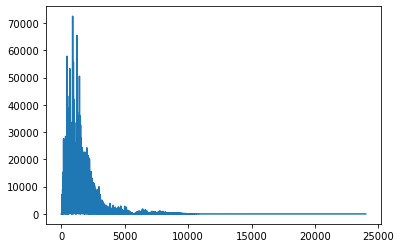
\includegraphics[width=0.75\textwidth]{1.png}
        \caption{2}
        \label{fig:first}
\end{figure}

Посмотрим на спектр: 

\begin{figure}[H]
        \centering
        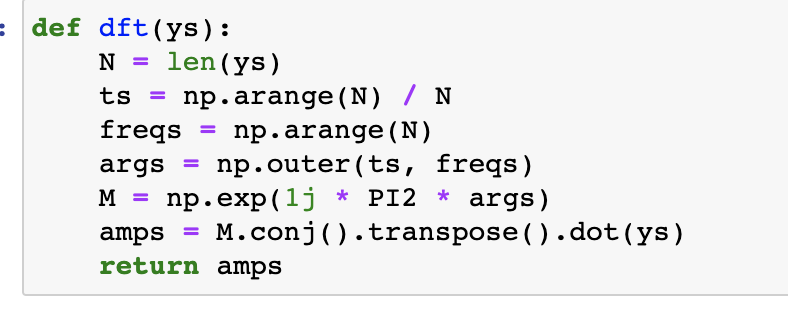
\includegraphics[width=0.75\textwidth]{2.png}
        \caption{2}
        \label{fig:first}
\end{figure}

Сделаем наложение пилообразного сигнала и прямоугольного:

\begin{figure}[H]
        \centering
        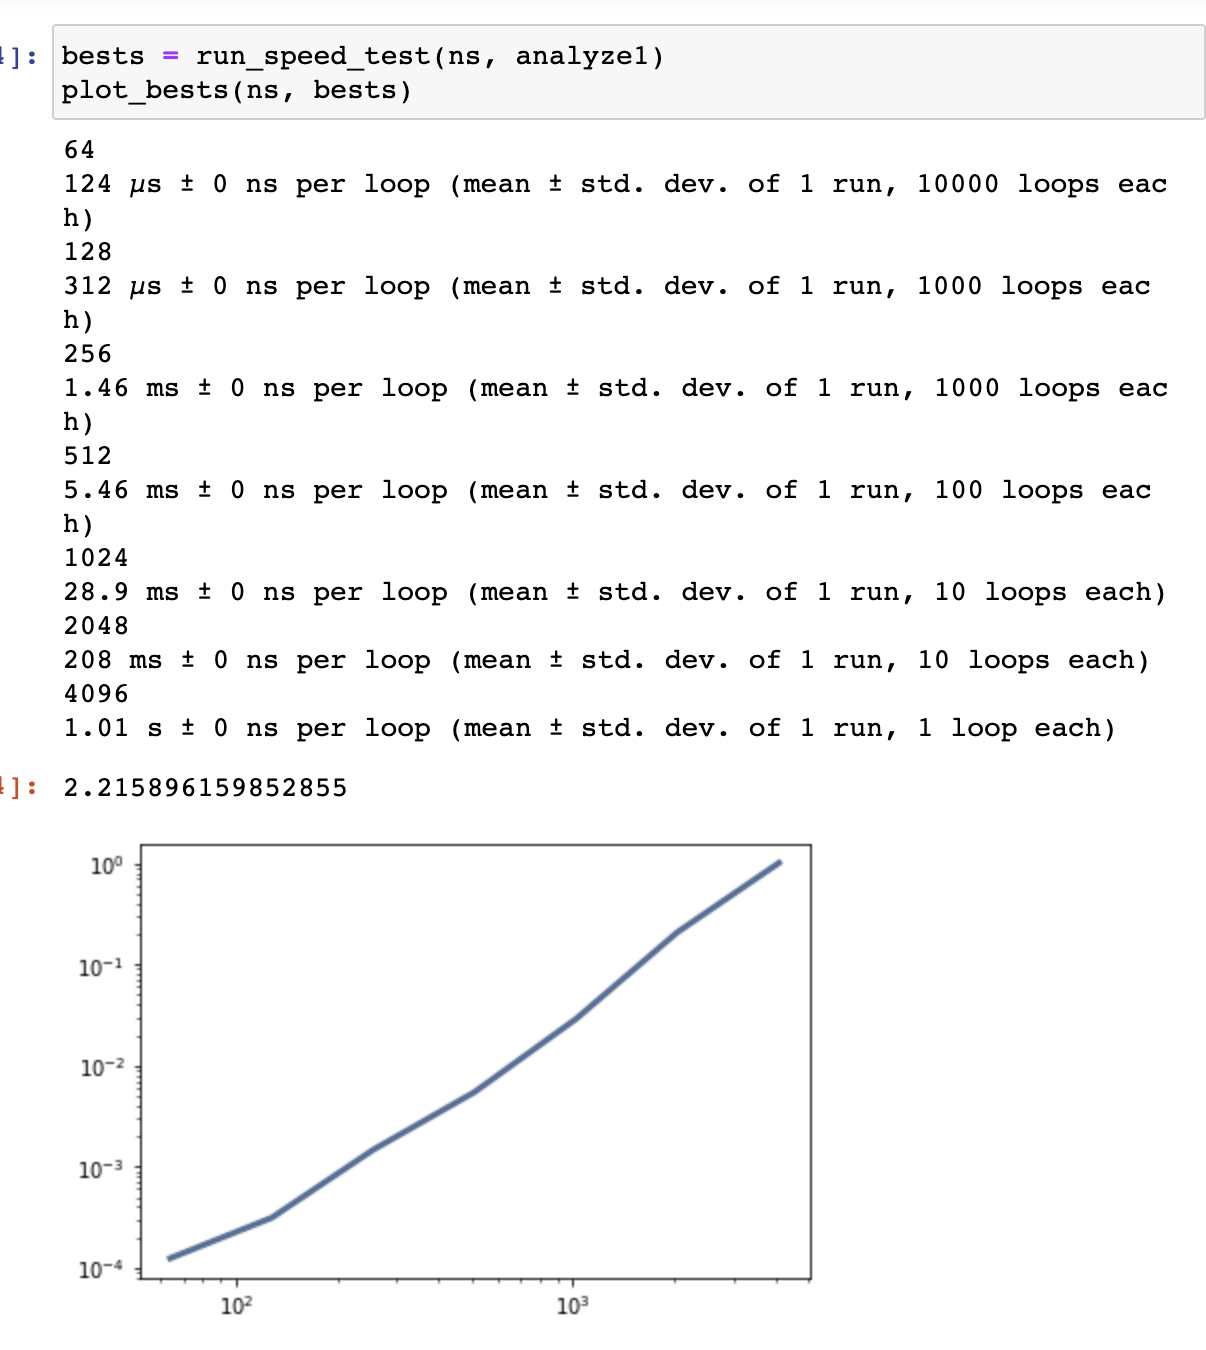
\includegraphics[width=0.75\textwidth]{3.png}
        \caption{2}
        \label{fig:first}
\end{figure}

Из графика видно, что спад пилообразных происходит аналогично спаду прямоугольных.

Также сделаем наложение пилообразного сигнала и треугольного: 

\begin{figure}[H]
        \centering
        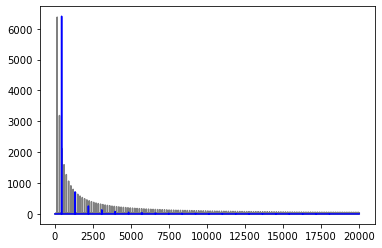
\includegraphics[width=0.75\textwidth]{4.png}
        \caption{2}
        \label{fig:first}
\end{figure}

В отличии от пилообразных гармоник, у треугольных спад протекает крайне быстро.
\section{Упражнение номер №2}
Необходимо создать прямоугольный сигнал 1100Гц и создать волну с выборками 10 000 кадров в секунду.  Построить спектр и убедиться, что большинство гармоник "завернуты" из-за биений. Проверить слышны ли последствия этого при проигрывании.

Создадим прямоугольный сигнал 1100Гц: 

\begin{figure}[H]
        \centering
        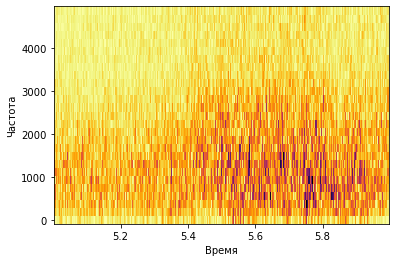
\includegraphics[width=0.75\textwidth]{5.png}
        \caption{2}
        \label{fig:first}
\end{figure}

Как видно из спектра, основная гармоника на частоте 1500 Гц и первуа гармоника на частоте 4500 Гц, но вторая гармоника, которая должна быть на частоте 7500 Гц, смещается на 2500 Гц. Третья гармоника, которая должна быть на частоте 10500 Гц, будет наложена на -500 Гц, но она снова будет наложена на 500 Гц.

\section{Упражнение номер №3}
Необходимо взять объект spectrum и распечатать несколько первых значений spectrum.fs . Убедиться что они начинаются с нуля. Затем нужно провести эксперименты:
1) Создать треугольный сигнал с частотой 440Гц и wave длительностью 0.01 секунд. Распечатать сигнал.
2) Создать объект spectrum и распечатать spectrum.hs[0]. Посмотреть каковы амплитуда и фазы этого компонента.
3) Установить spectrum.hs[0] = 100. Проверить как эта операция влияет на сигнал. 

Создали треугольный сигнал и посмотрели график сигнала:

\begin{figure}[H]
        \centering
        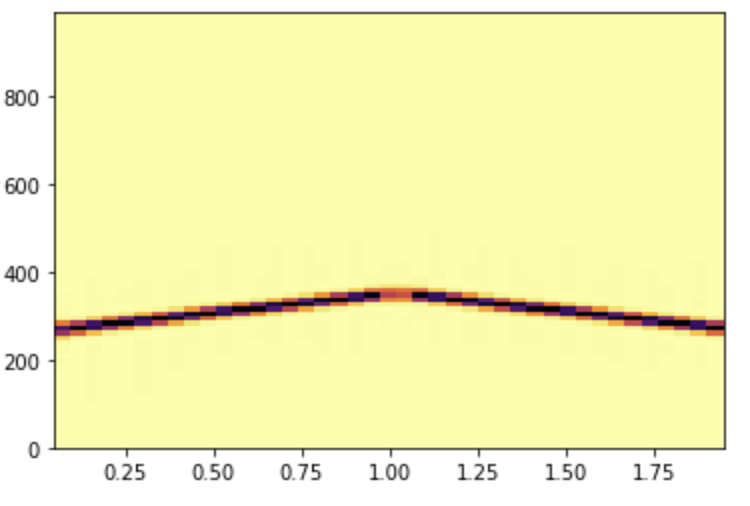
\includegraphics[width=0.75\textwidth]{6.png}
        \caption{2}
        \label{fig:first}
\end{figure}

Каждый элмент массива hs объекта Spectrum представялет собой комплексное число и соответствует частотоной компоненте: размах пропорционален амплитуде соответствующей компоненты, а угол - это фаза. Как видно из результатов выполнения кода, первый элемент массива hs - комплексное число, близкое к нулю, мнимая часть равна нулю. Присвоим первый элемент 100 и посмотрим, что из этого выйдет.

\begin{figure}[H]
        \centering
        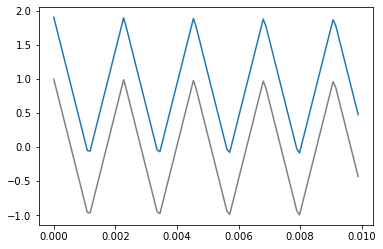
\includegraphics[width=0.75\textwidth]{7.png}
        \caption{2}
        \label{fig:first}
\end{figure}

Как мы можем заметить, добавляя компонент нулевой частоты мы можем сместить волну вертикально

\section{Упражнение номер №4}
Необходимо реализовать функцию, которая в качестве аргумента принимает spectrum и изменяет его делением каждого элемента hs на соответствующую частоту из fs. Проверить эту функцию на прямоугольном, треугольном и пилообразном сигналах:
1) Вычислить spectrum и распечатать его
2) Изменить spectrum и распечатать его
3) Использовать spectrum.make_wave, чтобы сделать wave из измененного spectrum, прослушать его. Посмотреть как изменился сигнал.

Реализуем метод

Создадим треугольный сигнал

Применим написанную нами функцию к созданному сигналу: 

\begin{figure}[H]
        \centering
        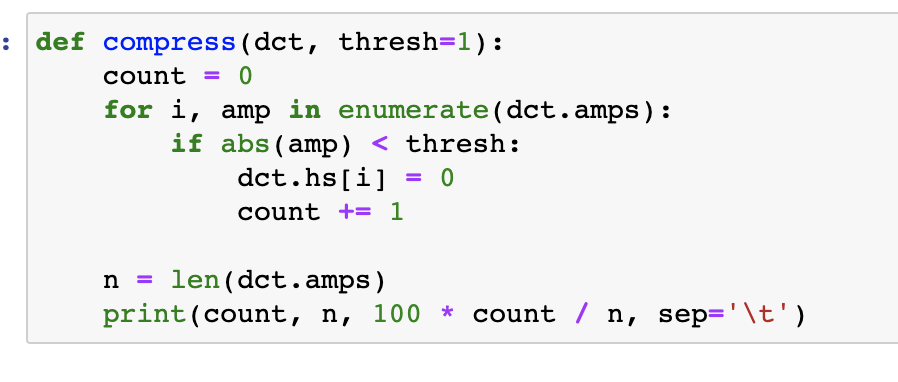
\includegraphics[width=0.75\textwidth]{8.png}
        \caption{2}
        \label{fig:first}
\end{figure}

Фильтр подавляет гармоники, поэтому он действует как фильтр нижних частот.
\section{Упражнение номер №5}
Проверить можно ли найти сигнал, состоящий из четных и нечетных гармоник, спадающих пропорционально 1/(f^2).

Нужно создать сигнал, состоящий из четных и нечетных гармоник, при этом, что эти гармоники падали пропорционально 1/ (f^2) Для этого воспользуемся одним из способов: создадим пилообразный сигнал и выведем его спектр:  

\begin{figure}[H]
        \centering
        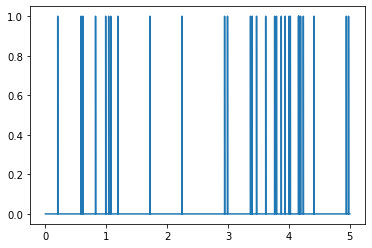
\includegraphics[width=0.75\textwidth]{9.png}
        \caption{2}
        \label{fig:first}
\end{figure}

Используем функцию из предыдущего пункта и преобразуем наш сигнал, а после сделаем наложение спектров: 

При наложении видно, что спад происходит как в условии

\begin{figure}[H]
        \centering
        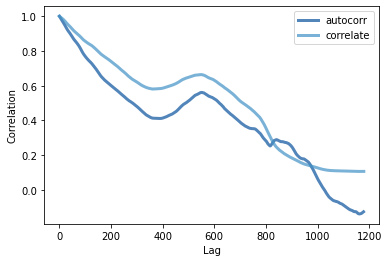
\includegraphics[width=0.75\textwidth]{10.png}
        \caption{2}
        \label{fig:first}
\end{figure}

Отобразим полученную нами wave:

\begin{figure}[H]
        \centering
        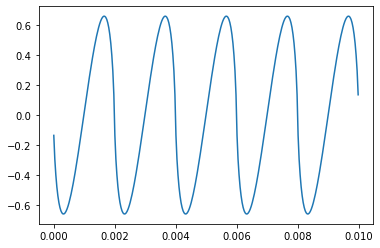
\includegraphics[width=0.75\textwidth]{11.png}
        \caption{2}
        \label{fig:first}
\end{figure}

Как видно из графиков, полученных после обработки сигнала, спектр спадает пропорционально как сказано в условии и при этом имеет четные и нечетные графики. Как видно из последнего графика, сигнал перестал быть пилообразным, и стал похожим на синусоидный.

\end{document}
